\section{Divine Spells}
Clerics, druids, experienced rangers, and templars can cast divine spells. Unlike arcane spells, divine spells draw power from a divine source. Clerics forge a pact with a particular element, and draw their power from the elemental planes themselves. Rangers learn to manipulate minor nature spirits, druids are granted their powers directly from the spirits of the lands, while templars are gifted with spell by their sorcerer-kings.

\subsection{Preparing Divine Spells}
Divine spellcasters prepare their spells in largely the same manner as wizards do, but with a few differences. The relevant ability for divine spells is Wisdom. To prepare a divine spell, a character must have a Wisdom score of 10 + the spell's level. Likewise, bonus spells are based on Wisdom.

\begin{figure*}[b!]
\centering
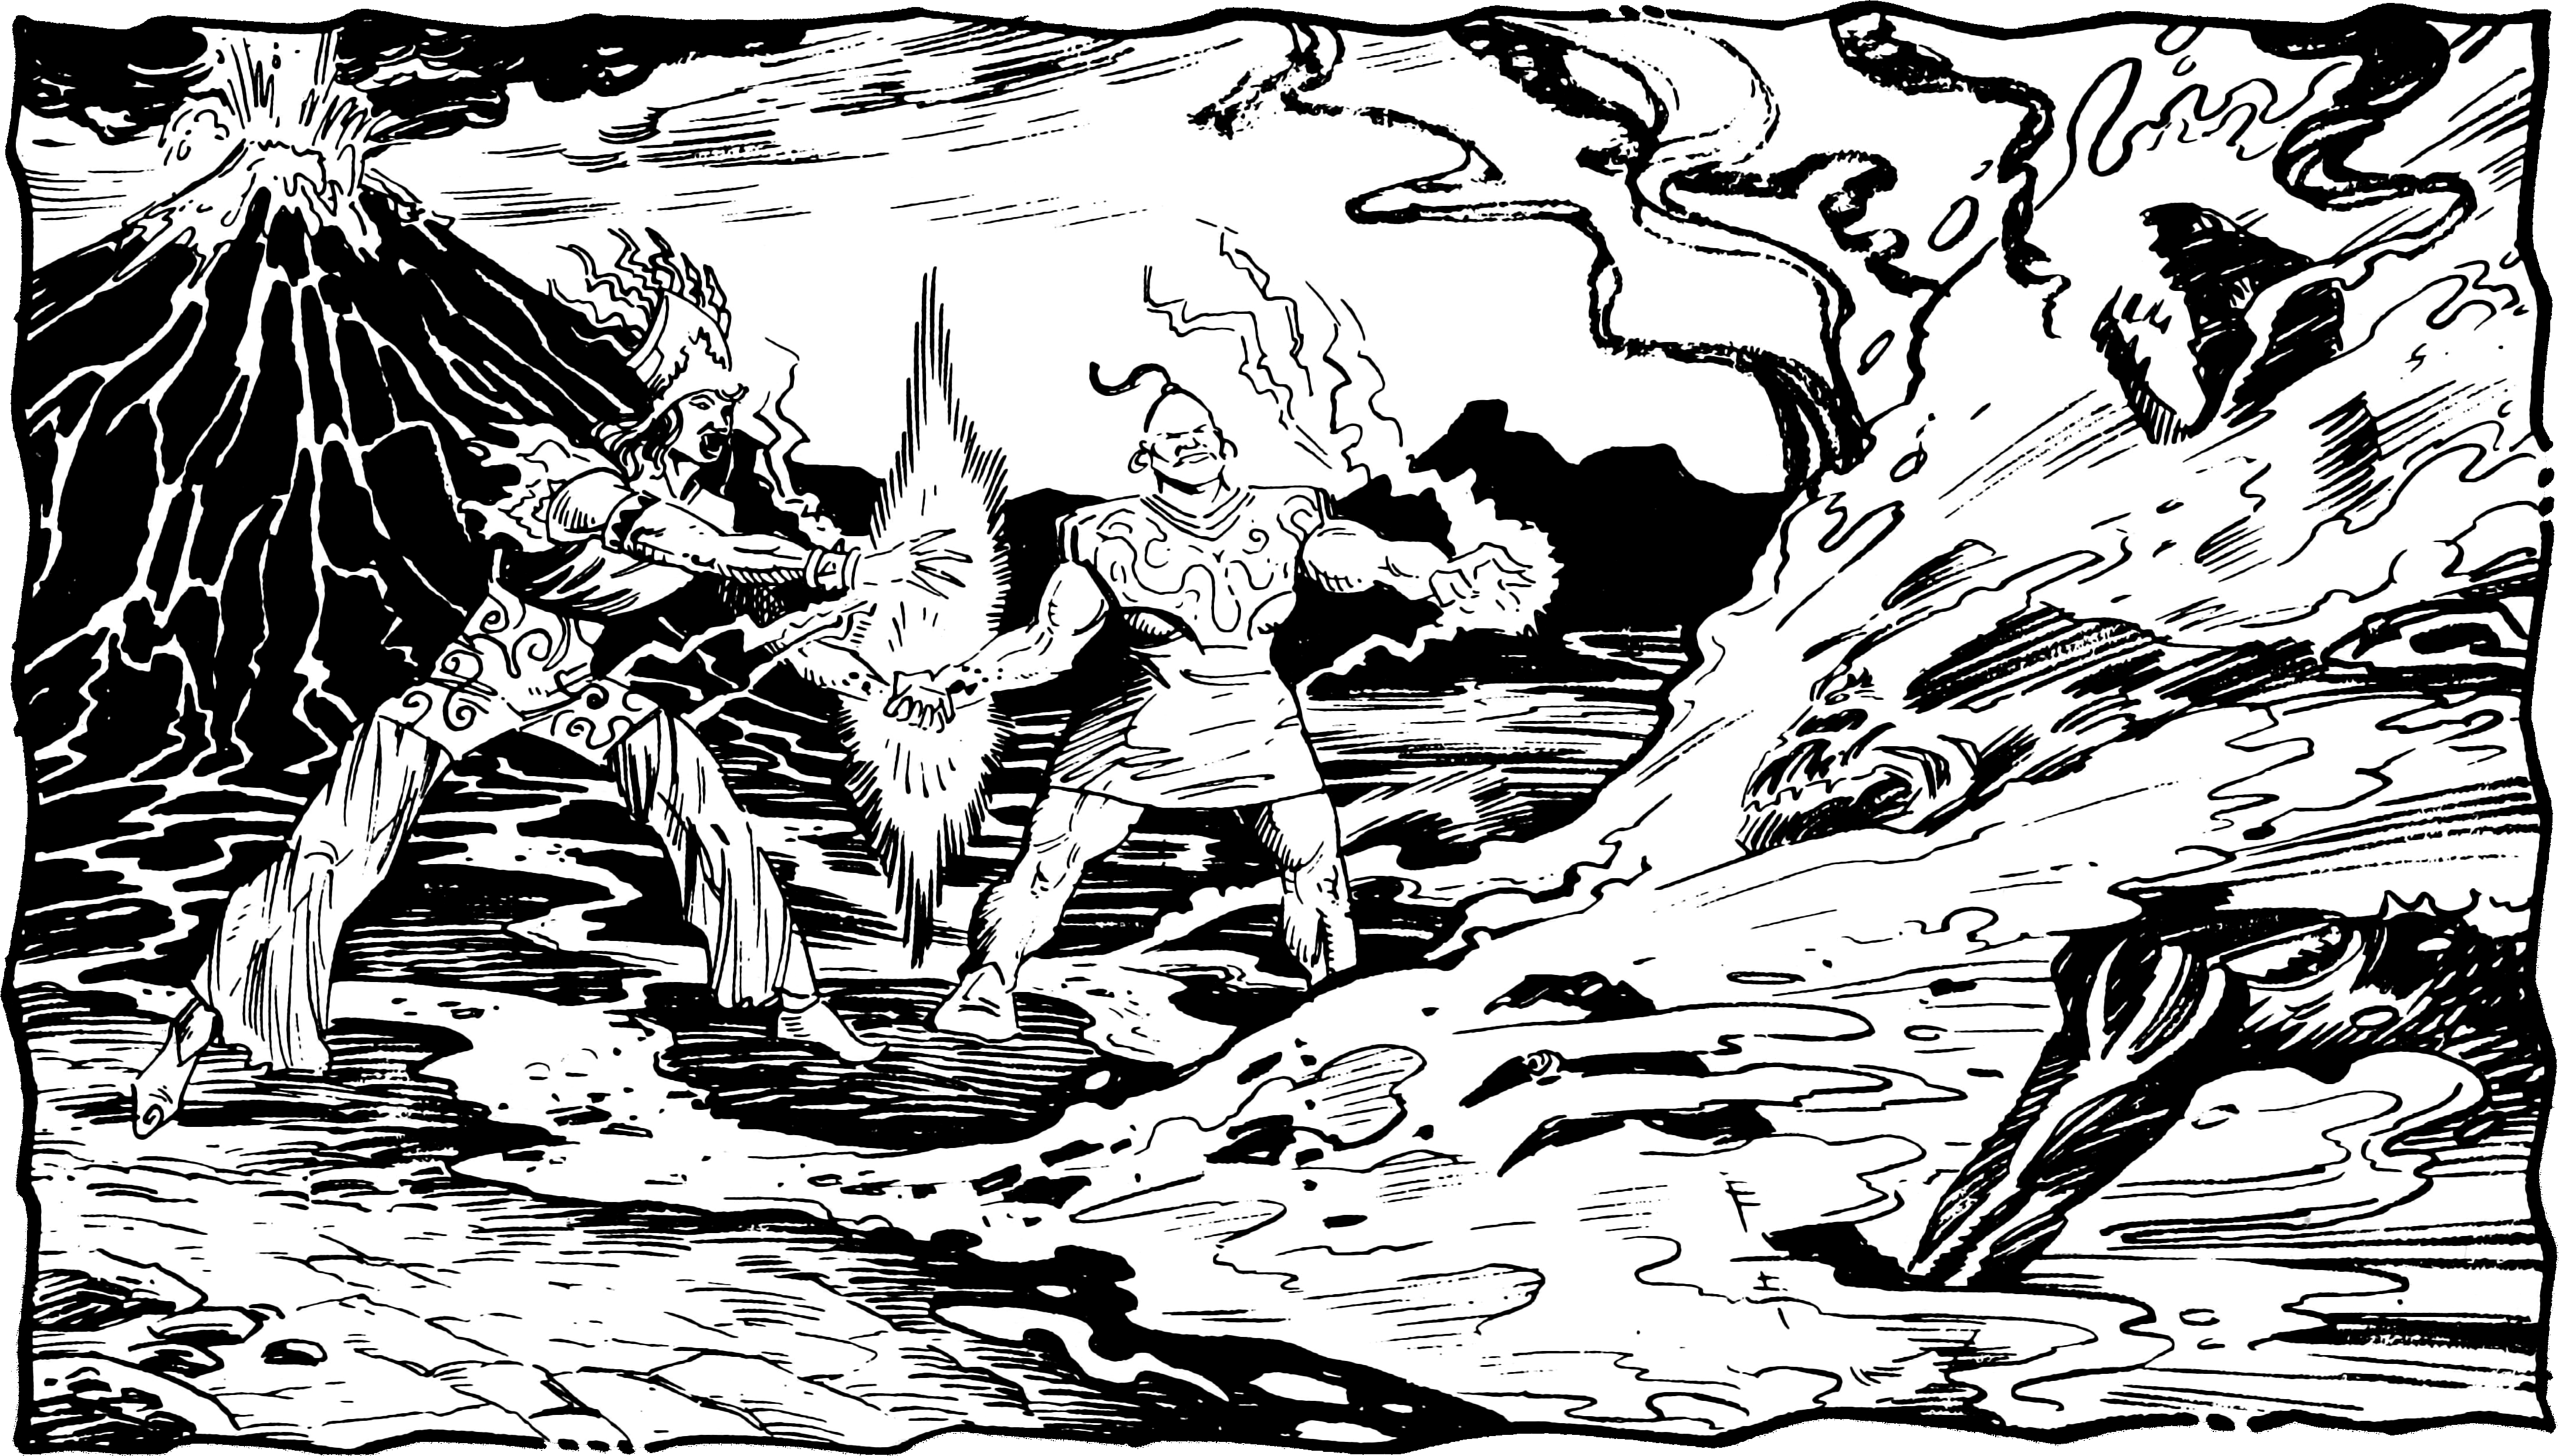
\includegraphics[width=\textwidth]{images/cleric-6.png}
\WOTC
\end{figure*}

\textbf{Time of Day:} A divine spellcaster chooses and prepares spells ahead of time, just as a wizard does. However, a divine spellcaster does not require a period of rest to prepare spells. Instead, the character chooses a particular part of the day to pray and receive spells. The time is usually associated with some daily event. If some event prevents a character from praying at the proper time, he must do so as soon as possible. If the character does not stop to pray for spells at the first opportunity, he must wait until the next day to prepare spells.

\textbf{Spell Selection and Preparation:} A divine spellcaster selects and prepares spells ahead of time through prayer and meditation at a particular time of day. The time required to prepare spells is the same as it is for a wizard (1 hour), as is the requirement for a relatively peaceful environment. A divine spellcaster does not have to prepare all his spells at once. However, the character's mind is considered fresh only during his or her first daily spell preparation, so a divine spellcaster cannot fill a slot that is empty because he or she has cast a spell or abandoned a previously prepared spell.

Divine spellcasters do not require spellbooks. However, such a character's spell selection is limited to the spells on the list for his or her class. Clerics, druids, rangers, and templars have separate spell lists. A cleric also has access to two domains determined during his character creation. Each domain gives him access to a domain spell at each spell level from 1st to 9th, as well as a special granted power. With access to two domain spells at each spell level---one from each of his two domains---a cleric must prepare, as an extra domain spell, one or the other each day for each level of spell he can cast. If a domain spell is not on the cleric spell list, it can be prepared only in a domain spell slot.

\textbf{Spell Slots:} The character class tables show how many spells of each level a character can cast per day.

These openings for daily spells are called spell slots. A spellcaster always has the option to fill a higher-level spell slot with a lower level spell. A spellcaster who lacks a high enough ability score to cast spells that would otherwise be his or her due still gets the slots but must fill them with spells of lower level.

\textbf{Recent Casting Limit:} As with arcane spells, at the time of preparation any spells cast within the previous 8 hours count against the number of spells that can be prepared.

\textbf{Spontaneous Casting of Cure and Inflict Spells:} A good cleric (or a cleric of a good deity) can spontaneously cast a cure spell in place of a prepared spell of the same level or higher, but not in place of a domain spell. An evil cleric (or a cleric of an evil deity) can spontaneously cast an inflict spell in place of a prepared spell (one that is not a domain spell) of the same level or higher. Each neutral cleric of a neutral deity either spontaneously casts cure spells like a good cleric or inflict spells like an evil one, depending on which option the player chooses when creating the character. The divine energy of the spell that the cure or inflict spell substitutes for is converted into the cure or inflict spell as if that spell had been prepared all along.

\textbf{Spontaneous Casting of Summon Nature's Ally Spells:} A druid can spontaneously cast a summon nature's ally spell in place of a prepared spell of the same level or higher. The divine energy of the spell that the summon nature's ally spell substitutes for is converted into the summon spell as if that spell had been prepared all along.

\subsubsection{Combined Casting}
Clerics of 7th level or higher can join forces to cast a spell from a paralemental domain. This special casting cannot be done by paraelemental clerics.

In order to cast this spell, the clerics must meet the conditions for casting:
\begin{itemize*}
\item The clerics must be in contact with the paraelements, or with each of their own elements.
\item The clerics must be in physical contact with each other, by joining hands for example.
\item Both clerics must perform whatever somatic, verbal, or material components necessary for the spell.
\item The spell's casting time is doubled (see \tabref{Combine Casting}).
\item Both clerics use the domain slot of that spell level.
\end{itemize*}

\Table{Combine Casting}{XX}{
\tableheader Original Casting Time & \tableheader New Casting Time\\
1 swift action & 1 move action \\
1 standard action & 1 full round \\
1 full round or longer & Double the time \\
}

If the clerics are of the same level but have different Wisdom modifiers, the spell DC is based on the lower modifier. If the clerics have different levels, the effects of the spell are based on the lower level cleric, such as the spell's range, damage, number of targets and the spell's DC.

For example, Herak is a 9th-level fire cleric and Tella is a 7th-level earth priest. They want to combine powers and cast a spell of the Paraelemental Plane of Magma. Since they are standing in a rich field, Tella is in contact with her element, but there is no fire. Herak casts \spell{continual flame} to create magical fire to surround them. The first condition is met.

They decide to use the \spell{oil spray} spell. The clerics link hands, point their fingers at a small patch of earth and watch as a fountain of flammable oil spouts up. Since \spell{oil spray} is a 4th-level spell, both of them use their domain spell slot of 4th-level. They can still cast more combined spells depending on the domain spell slots available for both of them.

\subsection{Templars}
Templars cast divine spells, but they do not prepare their spells. A templar's class level limits the number of spells he can cast. %His high Charisma score might allow him to cast a few extra spells. A templar must have a Charisma score of at least 10 + a spell's level to cast the spell.

\textbf{Daily Readying of Spells:} Each day, templars must focus their minds on the task of casting their spells. A templar needs 8 hours of rest (just like a cleric), after which he spends 15 minutes concentrating. During this period, the templar readies his mind to cast his daily allotment of spells. Without such a period to refresh himself, the character does not regain the spell slots he used up the day before.

\textbf{Recent Casting Limit:} As with clerics, any spells cast within the last 8 hours count against the templar's daily limit.

\textbf{Adding Spells to a Templar's Repertoire:} A templar gains spells each time he attains a new level in his class and never gains spells any other way. Templars automatically know all spells on the templar's spell list, for each spell level they can cast. With permission, templars can also select the spells they gain from new and unusual spells that they have gained some understanding of.

\subsection{Divine Magical Writings}
Divine spells can be written down and deciphered just as arcane spells can (see Arcane Magical Writings). Any character with the \skill{Spellcraft} skill can attempt to decipher the divine magical writing and identify it. However, only characters who have the spell in question (in its divine form) on their class spell list can cast a divine spell from a scroll.

\subsection{New Divine Spells}
Divine spellcasters most frequently gain new spells in one of the following two ways.

\textbf{Spells Gained at a New Level:} Characters who can cast divine spells undertake a certain amount of study between adventures. Each time such a character receives a new level of divine spells, he or she learns new spells from that level automatically.

\textbf{Independent Research:} A divine spellcaster also can research a spell independently, much as an arcane spellcaster can. Only the creator of such a spell can prepare and cast it, unless he decides to share it with others.